\newpage

\section{Network Address Translation}
% https://www.youtube.com/watch?v=IsUFzuhwsME
NAT (Network Address Translation) can be explained as a part of the firewall that modifies packets so it reaches a specific address in a local network. This is the method that is used when you only have one IP on your WAN interface and all of the local IPs can communicate via that IP to the rest of the world. Most often, NAT is also changing the port numbers.

Learning objectives for this module:
\begin{itemize}
    \item How NAT is implemented.
    \item Port forwarding.
    \item NAT and IPv6.
\end{itemize}

In \opnsense\, there are four different settings/types of NAT that can be changed. Going through some of them in the next chapters. Use the menu; \cmd{Firewall --> NAT} to access the different types. The different types that \opnsense\ offers is, outbound, port forwarding, one-to-one, and NPTv6. The two last ones are not explained in this tutorial.

%The first part, outbound NAT (\ref{outbound}) is not relevant for the work done in this tutorial, since the automatic mode is working as intended. If you have free time during the tutorial session, try to make a rule that is working. The last part, NPTv6 (\ref{nptv6}) is not explained in this tutorial, since IPv6 is not used in it.

\begin{importantblock}
    Before starting on any of the configurations below, create snapshots of your \opnsense\ firewall or create a backup of your configuration, so it is easy to restore it if errors are made.
\end{importantblock}

\subsection{Outbound}\label{outbound}
This is the most simple implementation of NAT, and it can be used in an automatic, manually or hybrid configuration. We are going to look at the manual mode here.
\tipbox{Manually configuration is needed when the ISP (Internet Service Provider) is providing a pool of IPs that can be used on the WAN side.}

In meny \cmd{Firewall --> NAT --> Outbound} the outbound NAT can be configured. The standard configuration can be seen in figure \ref{opnsense:nat_simple_outbound}.

\begin{figure}[h!]
    \centering
    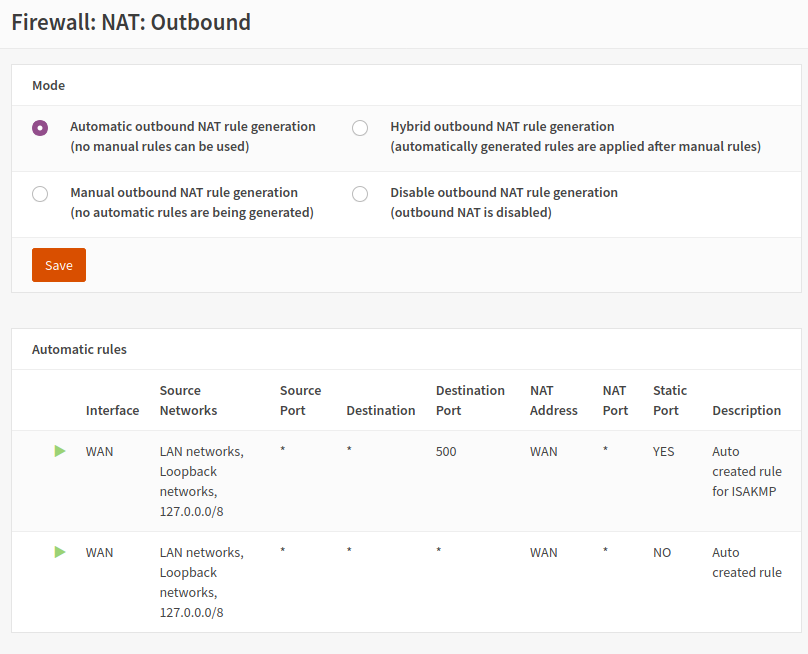
\includegraphics[width=0.7\textwidth]{Images/nat/nat_outbound.PNG}
    \caption{NAT Simple outbound NAT}
    \label{opnsense:nat_simple_outbound}
\end{figure}

To change from the automatic to manual follow the steps below: 
\setupblock{\begin{enumerate}
    \item Click the box besides \cmd{Manual outbound NAT rule generation.}
    \item Click on \cmd{save}.
    \item Create a new rule and set the configuration to:
    \begin{enumerate}
        \item \cmd{Interface} to the WAN interface you are using.
        \item \cmd{TSP/IP Version} to \cmd{IPv4}.
        \item \cmd{Protocol} to \cmd{any}.
        \item \cmd{Source invert} no check mark in the box.
        \item \cmd{Source address} to \cmd{192.168.20.0/24}.
        \item \cmd{Source port} to \cmd{any}.
        \item \cmd{Destination invert} no check mark in the box.
        \item \cmd{Destination address} to \cmd{any}.
        \item \cmd{Destination port} to \cmd{any}.
        \item \cmd{Translation / target} to \cmd{Interface address}.
    \end{enumerate}
\end{enumerate}}

\quesblock{\begin{enumerate}
    \item[24.] What is outbound NAT?
    \item[25.] Is it working? 
\end{enumerate}}

\warnblock{The following step is not required since our network does not have multiple WAN addresses.}

If there is a pool of WAN addresses, either physical network adapters or virtual addresses, there are three changes that are needed in the configuration over. The first one is to change the \cmd{Translation / target} to the physical network adapters or virtual addresses. The second change is to choose how the firewall should choose which WAN IP is going to be used. This is done in the \cmd{Pool Option}. There are four different methods to choose from:
\begin{itemize}
    \item Random - Random select an IP in the pool.
    \item Round Robin - This is the default option. Loops through the IPs in the pool.
    \item Source hash - Hashes the source address to ensure that the translation is correct.
    \item Bitmask - Keeps the last portion identical (\cmd{10.0.0.10 --> X.X.X.10}).
\end{itemize}

\warnblock{If your setup is using aliases, only Round Robin can be used.}

The last one is to create a firewall rule that is passing through the traffic.

\subsection{Port Forwarding} \label{port_forwarding}
The port Forward NAT method is used when you want to expose an internal service to the world. This could be a web server, email server or in a home network for example your Xbox console. In this tutorial, we are forwarding a simple python web server on port 8080 on the Ubuntu server. This web server will be accessible from your client machine when you are done with the configuration.

To set it up, follow the guide below:
\setupblock{\begin{enumerate}
    \item Go to \cmd{Firewall --> NAT --> Port forward}
    \item Click on \cmd{add}.
    \item Configure:
    \begin{enumerate}
        \item Set \cmd{Interface} to WAN.
        \item Set \cmd{TSP/IP Version} to \cmd{IPv4}.
        \item Set \cmd{Protocol} to \cmd{TCP}.
        \item \cmd{Destination invert} no check mark in the box.
        \item Set \cmd{Destination} to \cmd{WAN address}.
        \item \cmd{Destination port range} to \cmd{other} and choose \cmd{8080} in both of the \cmd{from} and \cmd{to} boxes.
        \item Set \cmd{Redirect target IP} to \cmd{192.168.20.12} (Check if this is your Ubuntu Server IP).
        \item Set \cmd{Redirect target port} to \cmd{8080}.
        \item Make a checkmark in the \cmd{Log} checkbox.
        \item Click \cmd{Save} and \cmd{Apply Changes}.
    \end{enumerate}
\end{enumerate}}

\subsection*{Creating and accessing a simple web server} \label{python_server}
Now the port forwarding is done, let's create a simple web server using Python. Python 3 should be preinstalled, if not use the command \cmd{sudo apt install python3} on the Ubuntu server to install it.

Configure the web server and creating the \cmd{index.html} file:
\setupblock{\begin{enumerate}
    \item In your home directory, on the Ubuntu server, create a new folder called \cmd{www}. Use the command: \cmd{mkdir www} to make it.
    \item Go to the directory using the command: \cmd{cd www}.
    \item Create a \cmd{index.html} file that returns a hello world when someone is acceesing it. This can be done using multiple methods: Below are two methods:
    \begin{itemize}
        \item Use this command: \cmd{echo "<h1>Hello World</h1>" > index.html}, or
        \item Use your favorite editor and insert the command \cmd{<h1>Hello World</h1>} on line one. (\cmd{nano and vim are installed on the Ubuntu server}) When \cmd{index.html} is opened in nano it should look like figure \ref{opnsense:nat_index}.
    \end{itemize}
\end{enumerate}}

\begin{figure}[h!]
    \centering
    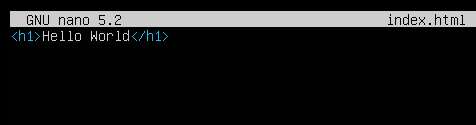
\includegraphics[width=0.5\textwidth]{Images/nat/index.PNG}
    \caption{index.html opened in nano}
    \label{opnsense:nat_index}
\end{figure}

The next step is to create the Python 3 web server on port 8080. This is done using the command:

\setupblock{\cmd{python3 -m http.server 8080}}

Now, try to access the webserver from your host machine. Open a browser and use the WAN address on your firewall and port 8080. You should get something like figure \ref{opnsense:nat_python_client}, but using your WAN IP address.

\begin{figure}[h!]
    \centering
    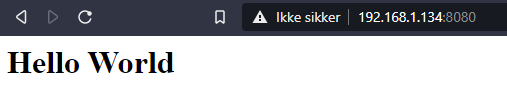
\includegraphics[width=0.6\textwidth]{Images/nat/client_browser.PNG}
    \caption{Accessing the simple web server from the host machine}
    \label{opnsense:nat_python_client}
\end{figure}

If you go to the Ubuntu Server you will see that the console output from the python webserver gives you an HTTP status code of 200 like figure \ref{opnsense:nat_python}.

\begin{figure}[h!]
    \centering
    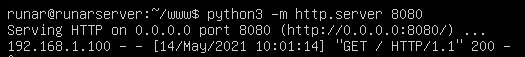
\includegraphics[width=0.6\textwidth]{Images/nat/python_server.PNG}
    \caption{Simple Python 3 server}
    \label{opnsense:nat_python}
\end{figure}

\quesblock{\begin{enumerate}
    \item[26.] What does port forward do?
    \item[27.] What can be done to improve the security when port forwarding is used?
\end{enumerate}}

\warnblock{The two sections below are only for information and for the student to explore.}

\subsection{One-to-one NAT} \label{one-to-one}
To set up a One-to-one NAT rule requires a three-step process. First, create a virtual IP (or use a physical network adapter), then create the NAT rule, and at last, create a firewall rule that can pass the traffic through.

\subsection{NPTv6} \label{nptv6}
IPv6 does not need to use NAT, since the address range is so large. But for load balancing, it can be smart to use NAT on IPv6.